% Overleaf-Datei, Spiegel in docs/overleaf/. Nur zusammen mit Overleaf aendern.
% Inhalt: Section 4.3 "Multireference geometries" (sec:mr-whynotmr, schliesst
% das OMol25-Kapitel ab) und Chapter 5 "Conclusion & Outlook" (ch:conclusion).
% Entwuerfe: docs/section_mr_outofscope.tex, docs/discussion_delta.md,
% docs/discussion_omol25.md.

\section{Multireference geometries: attempted, out of scope}
\label{sec:mr-whynotmr}

Multireference geometries and energies were attempted for these reactions
because they would be the gold standard for reactions with high
multireference character. They were placed out of scope. Problems arose,
and they are not needed for the question of this thesis: the models were
trained on \mbox{$\omega$B97M-V/def2-TZVPD} and are trying to find the
transition states of that surface, so the reference stays at that level.
A reference closer to the exact surface would answer a different
question, and a model agreeing with it would be right for the wrong
reason. No multireference barrier enters this work.

\paragraph{The overall problem: active space selection.} Every
multireference method needs an active space, and the result depends on
it. autoCAS~\cite{stein2019autocas} selects the space from a DMRG
calculation over all valence orbitals, which was not practical for
molecules of this size. AVAS~\cite{sayfutyarova2017} and selection by
hand require experience that could not be acquired within the time of
this work. A smaller choice of molecules for this part of the test set
would have avoided this. This is also why the standard protocol, NEVPT2
energies on unrestricted geometries, was not carried out.

\paragraph{The additional problem for geometries: active space
consistency.} Starting from the DFT transition state, AVAS selected a
space, CASSCF optimised a transition state with it, and AVAS at the
optimised geometry returned a different space. The geometry had been
optimised on a surface that does not belong to it. A possible solution is
an iteration:

\begin{enumerate}
  \item select the active space, with autoCAS where affordable;
  \item optimise the transition state at the CASPT2 or NEVPT2 level;
  \item re-select the active space at the optimised geometry;
  \item repeat until the selected space is the one the geometry was
    optimised with;
  \item add the next orbitals to the converged space and check that the
    result does not change.
\end{enumerate}

The re-selection in the optimised orbital basis is what the autoCAS
authors recommend for a single structure~\cite{stein2019autocas}; the
iteration above applies it to a moving geometry.

Significant time of this work went into this attempt. To the author's
knowledge, transition-state geometries optimised at a multireference
level do not exist as a benchmark set, which is why it was worth trying
and is documented here.

\chapter{Conclusion \& Outlook}
\label{ch:conclusion}

We return to Chapter~\ref{ch:delta} and RQ1, whether a model can be
lifted to a higher level of theory by relabelling only a subset of its
training data. The answer is yes, certainly as long as the spin
formalism is not changed with the labels, and Allen et
al.~\cite{allen2026} and DeePEST-OS~\cite{ren2026} have shown the same
at scale. Three things are certain. The correction reaches the higher
level of theory on the low-MR reactions, where the restricted solution
is the ground state: the barrier error drops to a third, in single
points and in searches the model drives itself, and the force error
drops to a third in every tier, with under 1\,\% of the dataset
relabelled. The correction does not change the quality of the
geometries: the transition states found with MACE+$\Delta$ lie as
close to the reference as those found with MACE (mean RMSD 0.054
against 0.056\,\AA, Figure~\ref{fig:rmsd-parity}). No improvement was
to be made here, since the transition states of
\mbox{$\omega$B97X-D3/6-31G(d)} and \mbox{$\omega$B97M-V/def2-TZVP}
lie within 0.007\,\AA{} of each other, below the geometry error of the
base model.

The correction is bounded by the base model. MACE alone misses its
own level by 42\,meV, that error enters MACE+$\Delta$ unchanged, and
the head cannot reduce it (Eq.~\eqref{eq:error-split}); the corrected
model ends at 56\,meV.

At mid and high multireference character the correction overshoots,
and Chapter~\ref{ch:mr} shows that the two tiers differ. In the mid
tier the restricted reference is the ground state at nine of ten
transition states, so the overshoot is the head's error. In the high
tier it is the ground state at only three of ten, so there the
reference itself was the wrong target.

Four changes could have made the correction better.

\begin{itemize}
  \item \textbf{A trainable encoder.} The head reads frozen features,
    which is why the baseline passes through. Unfreezing the last MACE
    layer or the readout on the same 80\,000 points would let the model
    move its own surface towards the target instead of adding an
    offset. The risk is forgetting the cheap-level surface where the
    relabelled points are sparse.
  \item \textbf{An input that sees the gap change.} The head predicts
    the difference from scalar features alone. A feature that tracks
    multireference character, such as $N_\text{FOD}$ or the
    $\langle S^2 \rangle$ of the label, would let the head learn that
    the gap shrinks instead of over-correcting.
  \item \textbf{Labels on the right surface.} Where the restricted
    solution is unstable, the head learns a difference between two
    restricted energies. Relabelling those points unrestricted, with a
    stability analysis, would give it a difference that describes the
    ground state.
  \item \textbf{A better base.} Every improvement of MACE on its own
    level transfers one to one, because that term passes through the
    sum unchanged.
\end{itemize}

The limits of this chapter are its 30 reactions, the restricted
treatment throughout, and def2-TZVP without the diffuse functions of
the target level.

The correction was not pushed further, because the principle had been
shown at scale by others~\cite{allen2026, ren2026}; the open question
was where relabelling stops, which is what Chapter~\ref{ch:mr} took up.

RQ2 asked whether a model can learn a surface from paths that were
never relaxed on that surface. The answer is only partly where the
surface has its saddle somewhere else than the path does, and that is
the case whenever relabelling changes the spin formalism. OMol25 is
that case: it relabelled the whole Transition1x set and moved the
labels from the restricted surface to the DFT ground-state surface,
using unrestricted DFT at \mbox{$\omega$B97M-V/def2-TZVPD}.
Chapter~\ref{ch:mr} shows the limit: unrestricted labels on paths that
were never re-optimised unrestricted contain no broken-symmetry saddle
geometry, so the models cannot learn where the saddle of that surface
lies. Figure~\ref{fig:pes} gives the intuition: a schematic of the
same geometries on the surface they were relaxed on and on the
surface they were labelled on.

\begin{figure}[t]
  \centering
  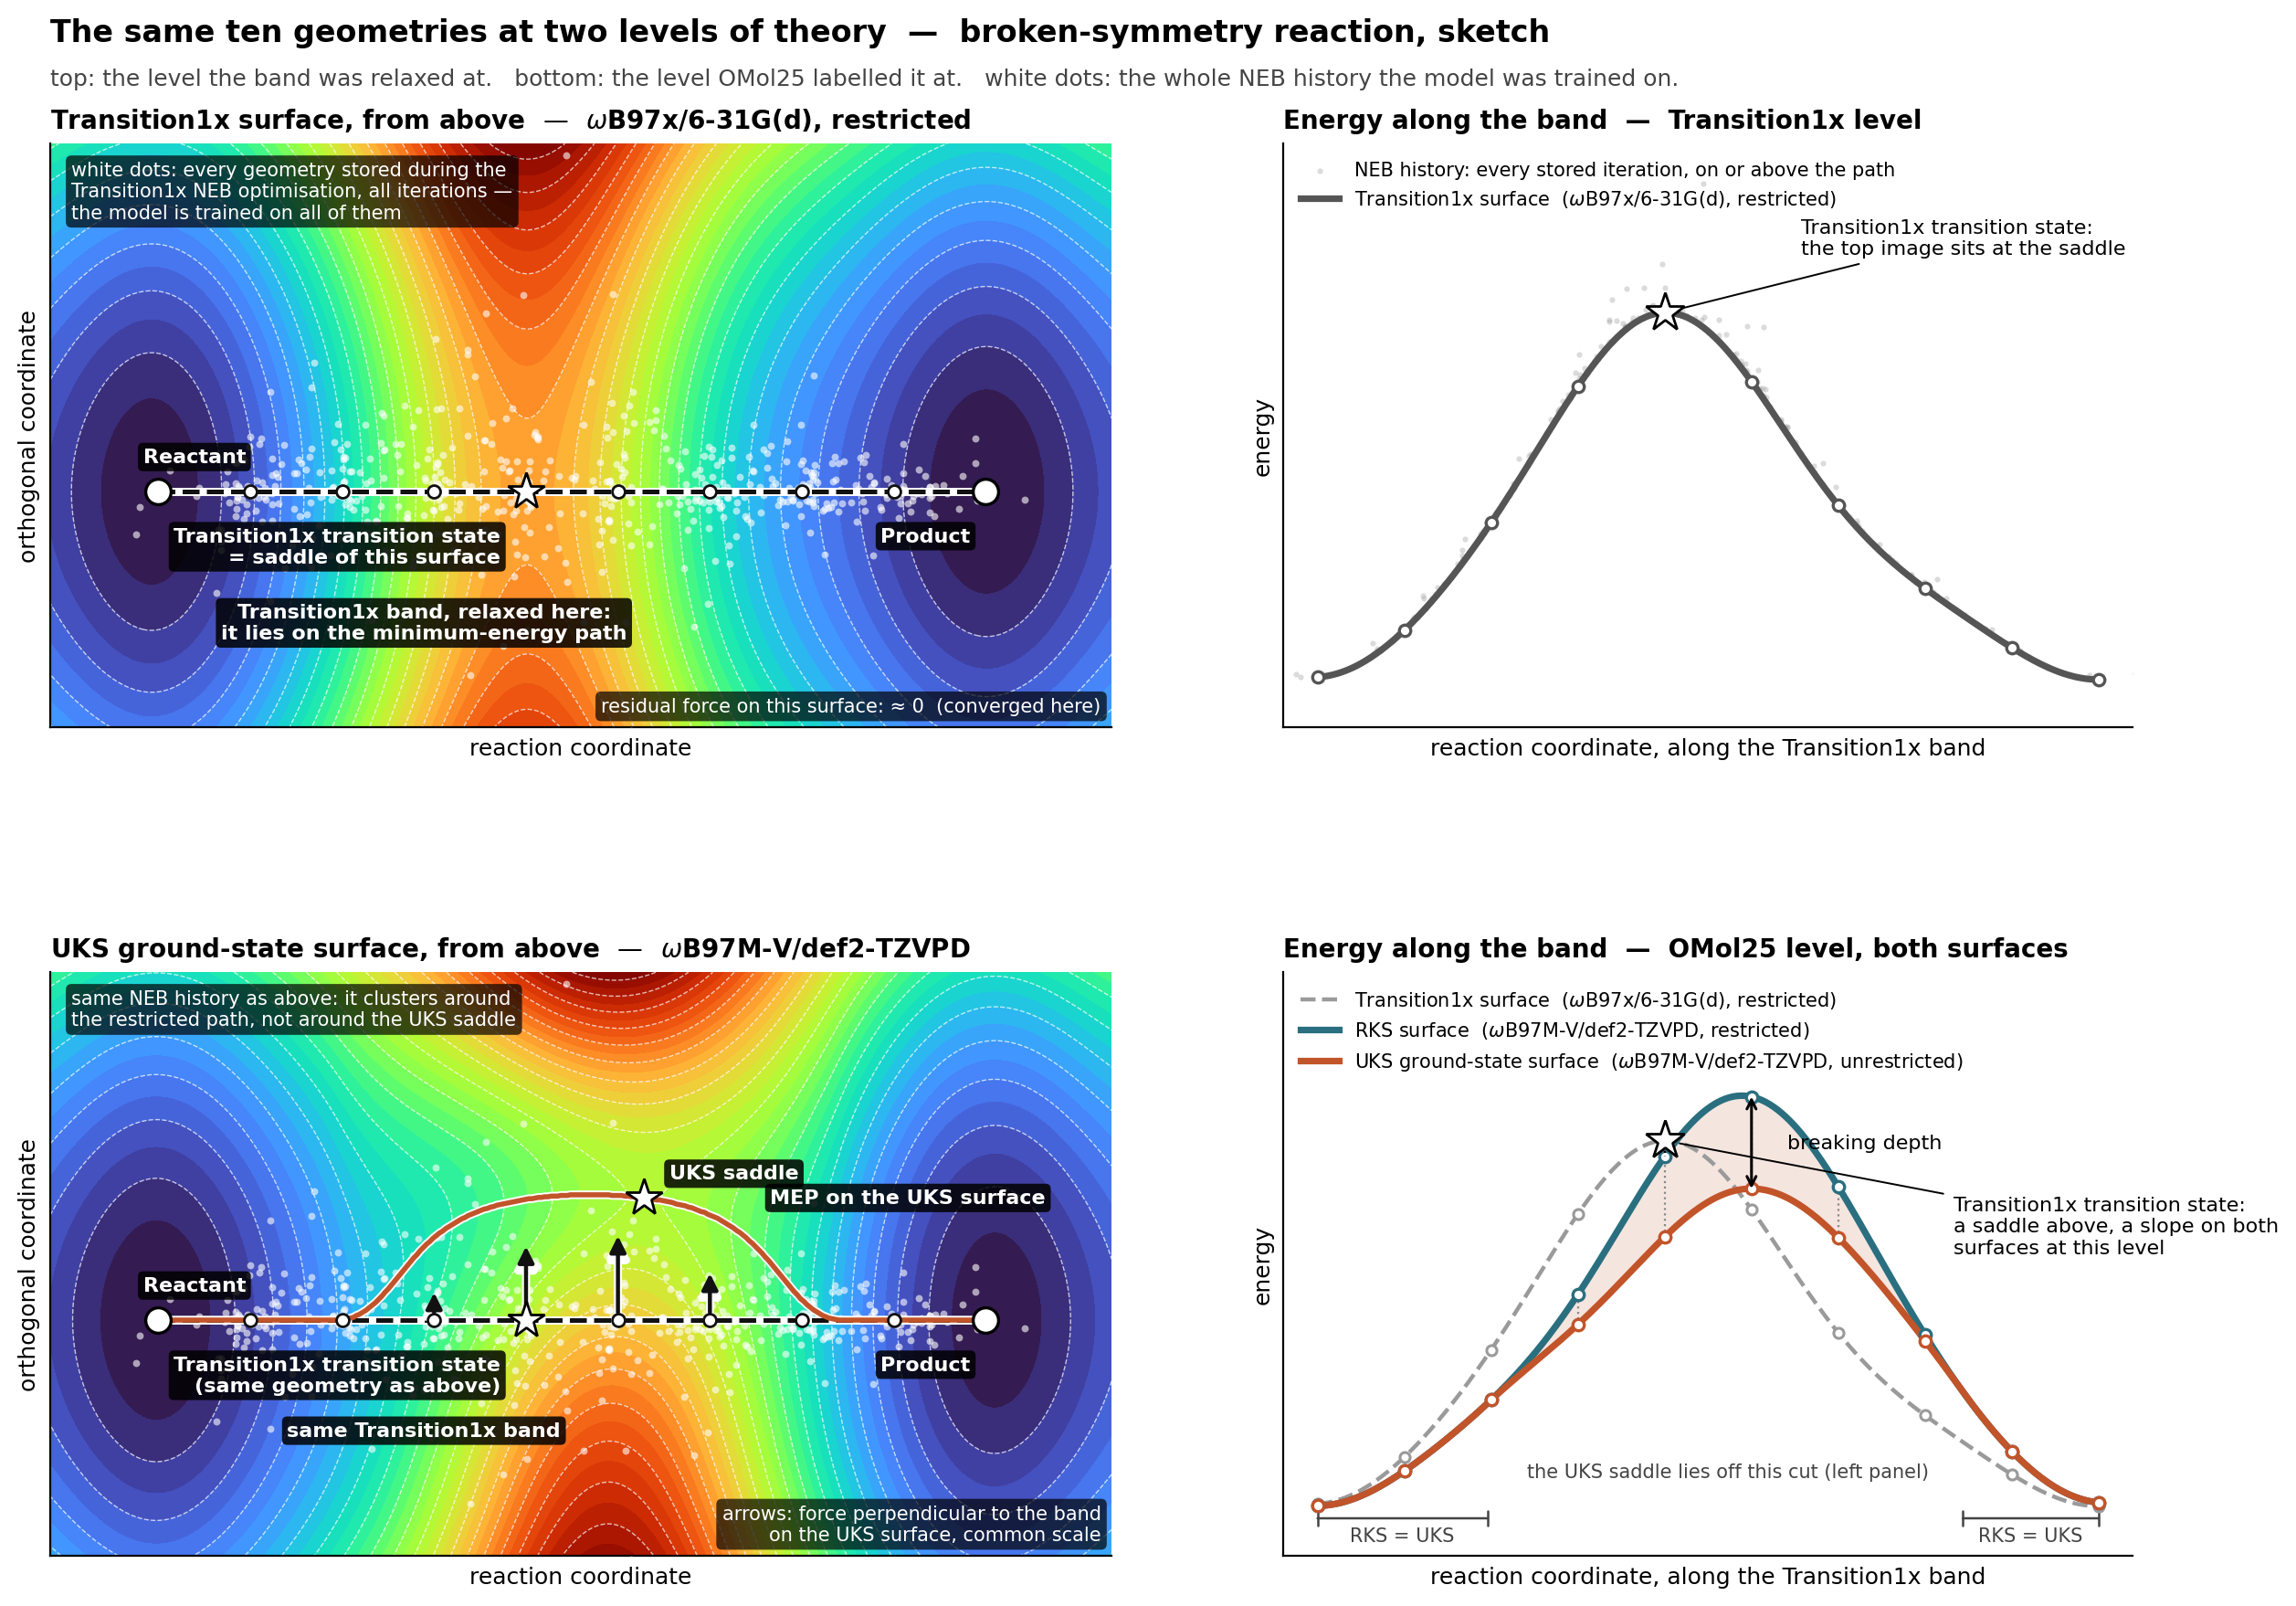
\includegraphics[width=\textwidth]{Pictures/fig_pes.png}
  \caption{Schematic of the mechanism, not a computed surface. The same
  geometries of a broken-symmetry reaction are shown on the restricted
  surface they were relaxed on (top) and on the ground-state surface
  they were labelled on (bottom). On the restricted surface the
  transition state is a saddle and the band with its stored NEB history
  (white dots) lies on the minimum-energy path. On the ground-state
  surface the same band lies on a slope, the force at the transition
  state is not zero (arrows), and the saddle lies elsewhere. Right: the
  energy along the band on each surface.}
  \label{fig:pes}
\end{figure}

Transition1x is not the only reactive data in OMol25, but no geometry
in OMol25 was relaxed at the level the labels use, and the other
organic reaction paths, Grambow and RGD1, were optimised restricted and
interpolated rather than relaxed~\cite{omol25}. A saddle of the
ground-state surface at the OMol25 level therefore does not exist
anywhere in the training data.

\paragraph{Unrestricted labels need new paths.} We therefore conclude that a
dataset like OMol25 is improved by adding paths relaxed on the surface
it labels with: one unrestricted CI-NEB per affected reaction, with a
stability analysis at the saddle to confirm that the path was relaxed
on the broken-symmetry surface and not on the restricted one, so that
the broken-symmetry transition states enter the training data as
stationary points.

\paragraph{Why the restricted default persists.} We see three possible reasons why
the field seems to overlook the unrestricted treatment when it builds
datasets and benchmarks:

\begin{itemize}
  \item it is the default: a quantum chemistry program runs a singlet
    restricted unless told otherwise, and nothing in a high-throughput
    workflow tells it otherwise;
  \item the alternative is expensive and fragile;
  \item nothing in the workflow reveals the problem.
\end{itemize}

The first needs no explanation. Regarding the second point: an
unrestricted path needs a stability analysis or a carried-over guess
at every image, the SCF solution changes character along the path, and
images fall back to the restricted solution or jump between broken
ones. The attempts of this work at broken-symmetry transition states
met each of these and produced no reference that could be trusted. The
third is what makes the default persist: a restricted saddle is a
valid stationary point, the band converges, the frequency calculation
shows one imaginary mode, the model trains, and a benchmark built the
same way scores it correct. The default fails only against a check
that nobody in the chain runs.

\paragraph{No benchmark until now has shown this error.} The benchmarks the models
are tested against are run restricted, even where they contain
reactions that should be treated unrestricted. The reference set of
\'Asgeirsson et al.~\cite{asgeirsson2021} holds 27 such reactions
among 121, which Hait et al. found when they re-optimised it
unrestricted and then removed~\cite{hait2025}. The benchmark of Marks
et al.~\cite{marks2026} holds one among 25, optimised restricted like
the rest (Appendix~\ref{app:marks}). If the reference saddle is
restricted, a model that finds the restricted saddle passes, even
where the restricted solution is not the ground state.

No benchmark exists that tests models at broken-symmetry transition
states. We see this as a gap in the literature: the reported success
rates were measured on restricted references, and it is easy to assume
that they hold for all transition-state searches. This work shows that
they do not. A set of saddles optimised on the broken-symmetry
surface and confirmed by a stability analysis would give future
models a benchmark to be tested against.

\paragraph{Recommendation: A stability analysis before trusting a saddle.} One unrestricted single point with a
stability analysis tells whether the restricted solution is the ground
state at a geometry, at the cost of one extra SCF. We recommend it at
every transition state that is trusted further, as a training point,
a reference, or a starting point, and whose multireference character
cannot be ruled out.

\paragraph{Limitations.} The sample is 45 reactions of small CHNO
molecules selected for multireference character; the findings concern
this class, not OMol25 as a whole. Of the four OMol25 models
benchmarked by Marks et al., three were tested here; MACE-OMol25, the
one with the highest success rate there, was not. This work contains no transition
state relaxed on the broken-symmetry surface, no multireference
reference (Section~\ref{sec:mr-whynotmr}), and no test of the models
after fine-tuning on such saddles.
